\documentclass{beamer}

\usepackage{float}
\usepackage{listings}
\usepackage{hyperref}
\usepackage{graphicx}
\usepackage{tikz,times}
\usepackage{amsmath}
\usepackage{xspace}
\usepackage{array}

\mode<presentation>
{
  \usetheme{Warsaw} 
  \setbeamercovered{transparent}
}

\AtBeginSection{
\begin{frame}<beamer>{Outline}
  \tableofcontents[currentsection,currentsubsection]
\end{frame}
}


\title[]{Deep Learning lab}
\subtitle{}

\author[Uni-Freiburg]{Mostafa Mohamed, Omar Kassem}
\date{\today}
\institute{Alberts-Ludwig Universt\"at Freiburg}

%\usecolortheme{Copenhagen}


%\usetheme{EastLansing}
\usepackage{natbib}
\bibliographystyle{apalike}
% make bibliography entries smaller
\renewcommand\bibfont{\scriptsize}
% If you have more than one page of references, you want to tell beamer
% to put the continuation section label from the second slide onwards
\setbeamertemplate{frametitle continuation}[from second]
% Now get rid of all the colours
\setbeamercolor*{bibliography entry title}{fg=black}
\setbeamercolor*{bibliography entry author}{fg=black}
\setbeamercolor*{bibliography entry location}{fg=black}
\setbeamercolor*{bibliography entry note}{fg=black}
% and kill the abominable icon
\setbeamertemplate{bibliography item}{}

\begin{document}

\begin{frame}
\titlepage
\end{frame}

\begin{frame}{Outline}
  \setcounter{tocdepth}{1}
  \tableofcontents
\end{frame}

\section{Introduction}
\begin{frame}{Problem Statement}
\begin{enumerate}
\item Visual planning imitating A*
\item Changing target
\end{enumerate}
\begin{figure}
        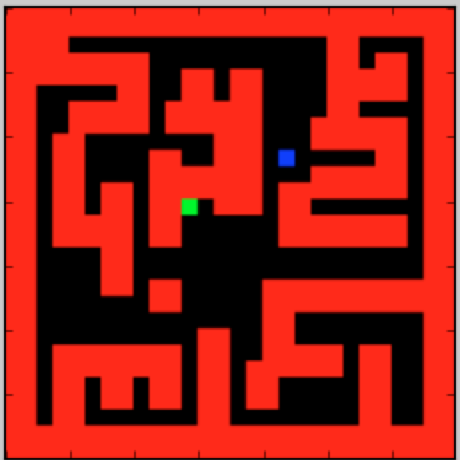
\includegraphics[width=0.30\linewidth]{problem.png}
    \label{fig1}
\end{figure}
\end{frame}

\section{Old results}
\begin{frame}{old results}
\end{frame}

\section{Storing target}
\begin{frame}{Adding target to state}
\end{frame}

\section{Coloring}
\begin{frame}{Simple coloring}
Average accuracy with colouring: 81\%

Average accuracy : 31\%
\begin{figure}
        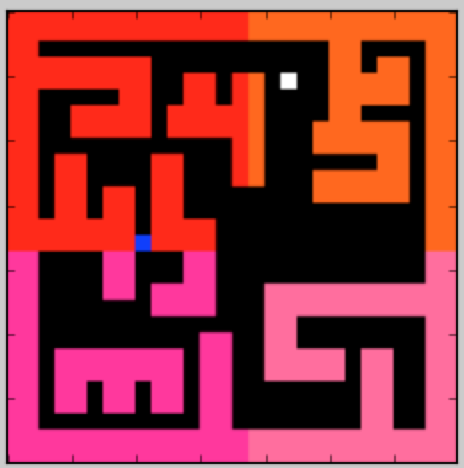
\includegraphics[width=0.35\linewidth]{simple.png}
        \caption{Simple colouring}
    \label{fig1}
\end{figure}
\end{frame}

\begin{frame}{Gradient coloring}
Average accuracy with colouring: 81\%

Average accuracy : 31\%
\begin{figure}
        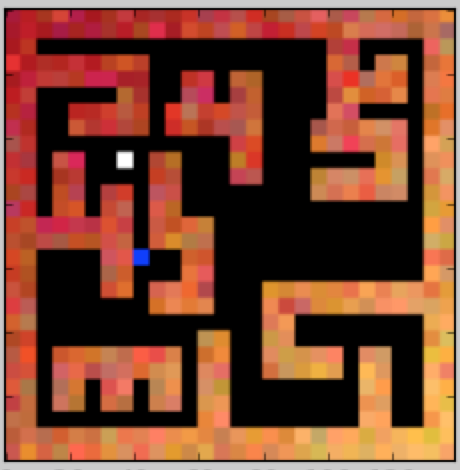
\includegraphics[width=0.35\linewidth]{gradient.png}
        \caption{Gradient colouring}
    \label{fig2}
\end{figure}
\end{frame}

\section{Gridding}
\begin{frame}{Distance accuracy}
\end{frame}

\begin{frame}{Gridding}
\end{frame}


\section{Final results}
\begin{frame}
\end{frame}

\iffalse
\begin{frame}{Recall}
\begin{figure}
        \includegraphics{train_test.png}
        \caption{Train and Test recall}
    \label{fig1}
\end{figure}
\end{frame}

\begin{frame}{Top 200 Recall}
\begin{figure}
        \includegraphics{recall200.png}
        \caption{Top 200 Recall}
    \label{fig1}
\end{figure}
\end{frame}

\begin{frame}{MRR, nDCG @ 5}
\begin{figure}
        \includegraphics{mrrndcg5.png}
        \caption{MRR, nDCG @ 5}
    \label{fig1}
\end{figure}
\end{frame}

\begin{frame}{MRR, nDCG @ 10}
\begin{figure}
        \includegraphics{mrrndcg10.png}
        \caption{MRR, nDCG @ 10}
    \label{fig1}
\end{figure}
\end{frame}
\fi



\end{document}
